\begin{frame}{CCSD $\op{T}_1$ amplitude equation }
    \note{Filename: ccsd\_diagramequations02.tex}

\begin{align*}
    0 &= 
    \parbox{10mm}{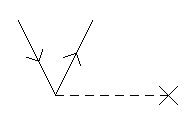
\includegraphics[scale=0.4]{graphics/ccsd_hbar_04a}}
    + \parbox{18mm}{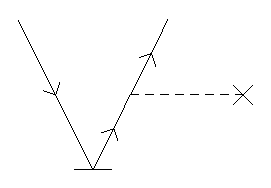
\includegraphics[scale=0.4]{graphics/ccsd_hbar_04b}}
    + \parbox{15mm}{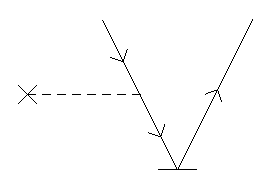
\includegraphics[scale=0.4]{graphics/ccsd_hbar_04c}}
    + \parbox{15mm}{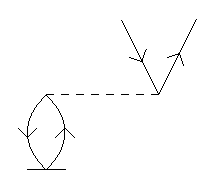
\includegraphics[scale=0.4]{graphics/ccsd_hbar_04d}} \\
    & \quad + \parbox{21mm}{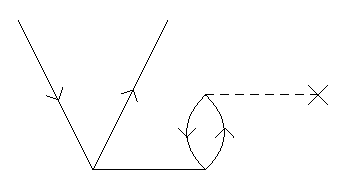
\includegraphics[scale=0.4]{graphics/ccsd_hbar_04e}}
    + \parbox{17mm}{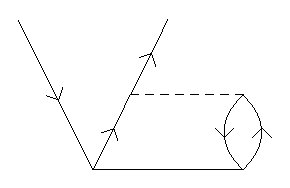
\includegraphics[scale=0.4]{graphics/ccsd_hbar_04f}}
    + \parbox{15mm}{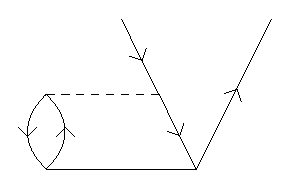
\includegraphics[scale=0.4]{graphics/ccsd_hbar_04g}}
    + \parbox{15mm}{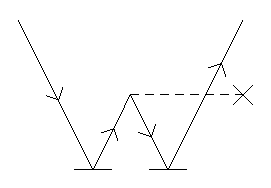
\includegraphics[scale=0.4]{graphics/ccsd_hbar_04h}} \\
    & \quad + \parbox{17mm}{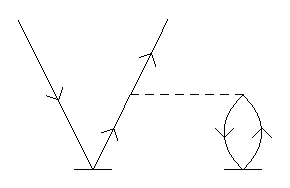
\includegraphics[scale=0.4]{graphics/ccsd_hbar_04i}}
    + \parbox{15mm}{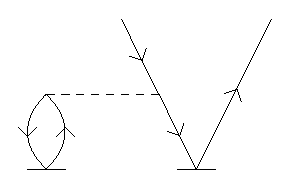
\includegraphics[scale=0.4]{graphics/ccsd_hbar_04j}}
    + \parbox{20mm}{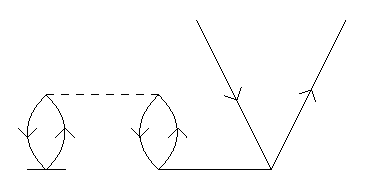
\includegraphics[scale=0.4]{graphics/ccsd_hbar_04k}}
    + \parbox{15mm}{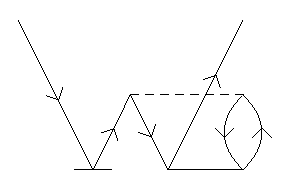
\includegraphics[scale=0.4]{graphics/ccsd_hbar_04l}} \\
    & \quad + \parbox{17mm}{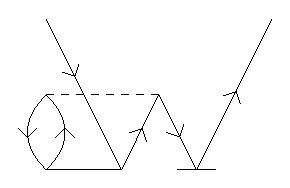
\includegraphics[scale=0.4]{graphics/ccsd_hbar_04m}}
    + \parbox{15mm}{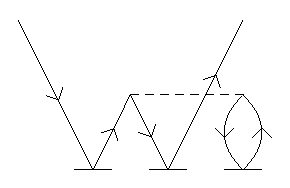
\includegraphics[scale=0.4]{graphics/ccsd_hbar_04n}}
\end{align*}

\end{frame}

    
